% TODO:
% --   domande età e primo approccio tecnologia, da vedere.
% --   da sistemare grafico età
% --   da sistemare grafico bravura pc (al posto di smartphone)
% --   cambiare titolo grafico età primo approccio tecnologia con:
%                "Età del primo approccio alla tecnologia"
% --   sistemare grafici uso app cucina
% --   sistemare anche usi app spesa
% --   dati incrociati e correlazioni
Per analizzare il target demografico per il quale viene effettuato lo studio dell'applicazione CookApp, 
si è effettuata un'analisi etnografica. Tale tipologia di analisi è fondamentale per ottenere dagli utenti
alcune informazioni fondamentali, di cui si terrà in seguito conto nella progettazione della UI e delle interazioni 
dell'applicazione. Al fine di ottenere informazioni sulla suddivisione demografica dei potenziali utenti, si è creato
un form anonimo tramite il software google forms\cite{GoogleModules}, che consente di creare, condividere ed analizzare in modo semplice
questionari di varia natura.

\subsection{Il sondaggio}
Il sondaggio proposto è composto da varie domande mirate alla
profilazione degli utenti a cui il progetto si relazionerà, vertendo
principalmente sull'enumerazione degli interessati in base a:
\begin{itemize}
	\item Età;
	\item sesso;
	\item relazione con la tecnologia;
	\item tecnologia con cui è stato effettuato il primo approccio;
	\item competenze culinarie;
	\item interesse e corrente utilizzo di applicazioni per il supporto alla
	cucina/spesa.
\end{itemize}

Per raggiungere tale scopo sono state poste le seguenti semplici domande a
risposta multipla.

\subsubsection{Domande relative al profilo sociale degli utenti}
\begin{quote}
	\textbf{Sesso}
\end{quote}
La domanda posta permette di individuare la percentuale di interesse in
relazione al sesso.  I risultati hanno rilevato un leggero vantaggio di persone
di sesso femminile partecipanti al sondaggio.

\begin{figure}[H]
	\centering
	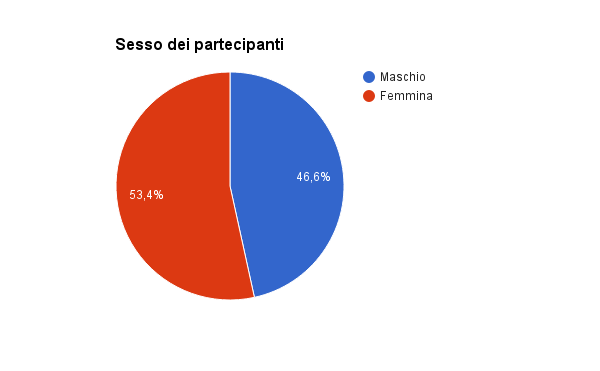
\includegraphics[scale=0.6]{img/chart_sesso}
\end{figure}

\begin{quote}
	\textbf{Età}
\end{quote}
Per individuare l'età media dell'utenza a cui ci rivolgeremo e per un'iniziale stima del livello
di competenza tecnologica che andremo ad affrontare le possibili risposte sono
state suddivise fasce:
\begin{itemize}
		\item Meno di 20 anni, ``nativi digitali", persone che si
			trovano a stretto contatto con i computer e gli
			smartphone moderni fin dai primi anni di vita.

		\item Da 20 a 30 anni, persone che hanno acquisito molta
			familiarità con il mondo tecnologico, principalmente
			grazie all'avvento dei videogiochi e le prime connessioni
			internet a banda larga.

		\item Da 30 a 40 anni, fascia composta da persone con molta conoscenza tecnica,
			legata principalmente al lavoro e alla cultura
			personale.

		\item Da 40 a 50 anni, come la fascia precedente, persone che
			sono state introdotte al mondo tecnologico non in età
			scolare.

		\item Da 50 a 60 anni, persone la quale familiarità tecnologica è
			stata introdotta durante la loro professione.
			Presentano inoltre piccoli disturbi legati all'età.

		\item Più di 60 anni, ``pensionati digitali",  persone il quale rapporto con la
			tecnologia avviene solamente per cultura personale e con
			notevoli disturbi legati all'età.
\end{itemize}

I risultati hanno evidenziato una discrepanza nel numero di partecipanti
relativi ad ogni fascia, con maggiori interessati nella fascia comprendente le
persone tra i 20 e i 30 anni.

\begin{figure}[H]
	\centering
	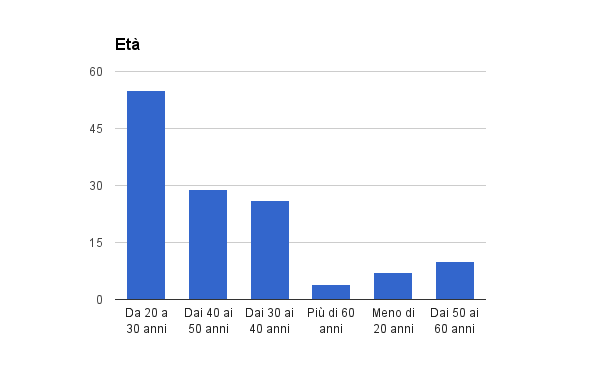
\includegraphics[scale=0.6]{img/chart_eta}
\end{figure}

\begin{quote}
	\textbf{Qual è il tuo livello di istruzione?}
\end{quote}
La domanda è utile per individuare la competenza di linguaggio degli utenti,
che, nel caso l'applicazione utilizzi termini troppo forbiti, potrebbe divenire
un ostacolo all'usabilità della stessa.  Anche in questo caso le risposte sono
state raggruppate in varie fasce:

\begin{itemize}
	\item Licenza elementare;
	\item licenza media;
	\item diploma di scuola superiore;
	\item laurea o superiore.
\end{itemize}
Anche in questo caso ,data anche l'età media dei partecipanti al sondaggio, è
sussistito uno squilibrio a vantaggio del diploma di scuola superiore.

\begin{figure}[H]
	\centering
	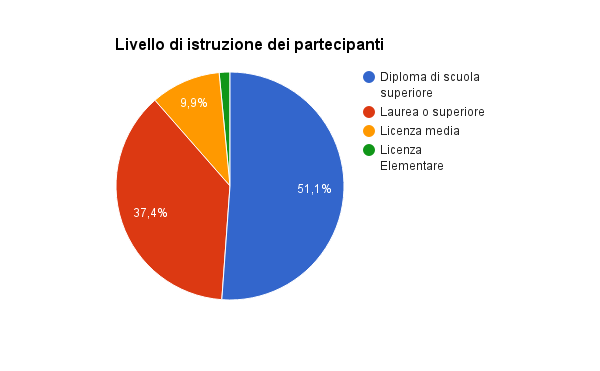
\includegraphics[scale=0.6]{img/chart_istruzione}
\end{figure}

\begin{quote}
	\textbf{Che lavoro fai?}
\end{quote}
In questo caso la domanda è utile sia per classificare il livello di competenza
linguistica degli utenti, sia per un'approssimativa stima della classe sociale
di questi ultimi. Purtroppo non è stato possibile porre la domanda in un modo
appropriato senza ottenere disturbi significativi da parte dei partecipanti.

\begin{itemize}
	\item Studente;
	\item operaio;
	\item impiegato;
	\item libero professionista;
	\item imprenditore;
	\item pensionato o casalinga;
	\item disoccupato.
\end{itemize}

Il numero degli studenti e impiegati è equiparabile, risultano
invece un po' meno presenti le altre categorie.

\begin{figure}[H]
	\centering
	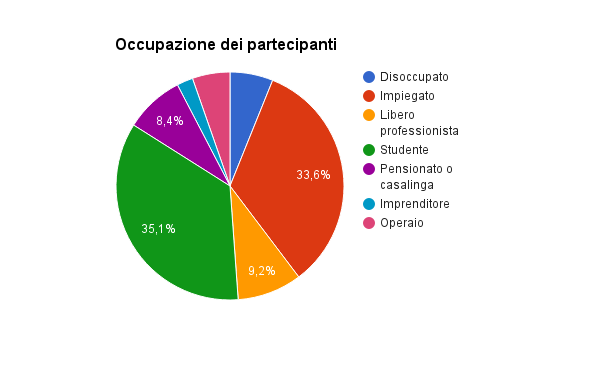
\includegraphics[scale=0.6]{img/chart_occupazione}
\end{figure}

\begin{quote}
	\textbf{Hai figli e/o nipoti? E se si, cucini per loro?}
\end{quote}

La presenza di un figlio implica la necessità di diversificare i piatti ed una
competenza di dominio più elevata rispetto alla media.\\

Dai grafici si deduce che la metà dei partecipanti possiede figli o nipoti, e
la maggior parte dei genitori cucina per i parenti.
\begin{figure}[H]
\centering
\begin{minipage}{.48\textwidth}
	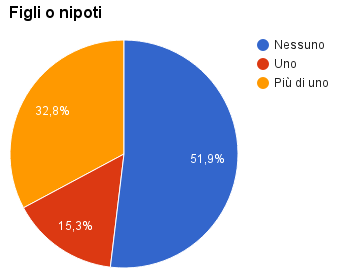
\includegraphics[scale=0.57]{img/chart_hai_figli_o_nipoti}
\end{minipage}
\hfill
\begin{minipage}{.49\textwidth}
	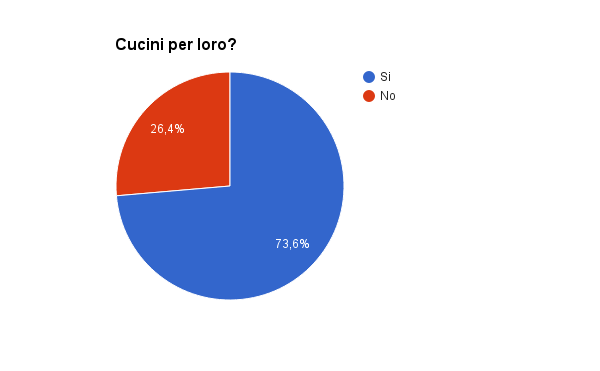
\includegraphics[scale=0.57]{img/chart_cucini_per_i_parenti}
\end{minipage}
\end{figure}

\subsubsection{Domande relative alle capacità tecnologiche degli utenti}
\begin{quote}
	\textbf{A che età hai avuto il primo approccio con la tecnologia?}
\end{quote}

Ricalcando la domanda posta per l'età del soggetto, vengono proposti i seguenti
scaglioni:

\begin{itemize}
	\item Fino a 6 anni;
	\item dai 6 ai 12 anni;
	\item dai 12 ai 20 anni;
	\item dai 20 ai 30 anni;
	\item dai 30 ai 50 anni;
	\item dopo i 50 anni.
\end{itemize}

Dal grafico si evince che la maggior parte degli utenti si è avvicinata alla
tecnologia durante la scuola dell'obbligo.  Ciò li rende tecnologicamente
competenti.
\begin{figure}[H]
	\centering
	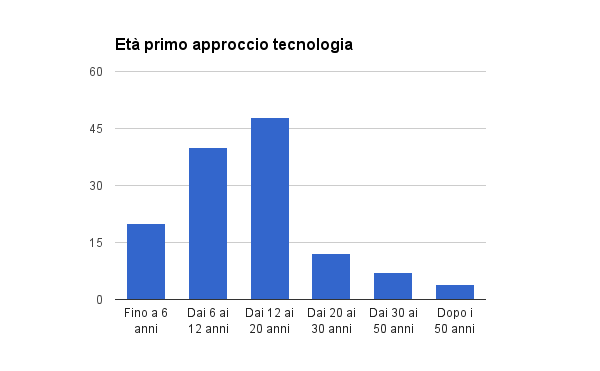
\includegraphics[scale=0.6]{img/chart_eta_primo_approccio}
\end{figure}

\begin{quote}
	\textbf{Con che genere di dispositivi?}
\end{quote}

Per migliorare l'analisi e collocare gli utenti nel giusto scaglione di
approccio alla tecnologia è stata chiesta loro la tipologia di dispositivo con
il quale sono entrati in questo mondo.

\begin{itemize}
	\item Computer;
	\item smartphone;
	\item tablet, proprio dei nativi digitali;
	\item altro .
\end{itemize}

\begin{figure}[H]
	\centering
	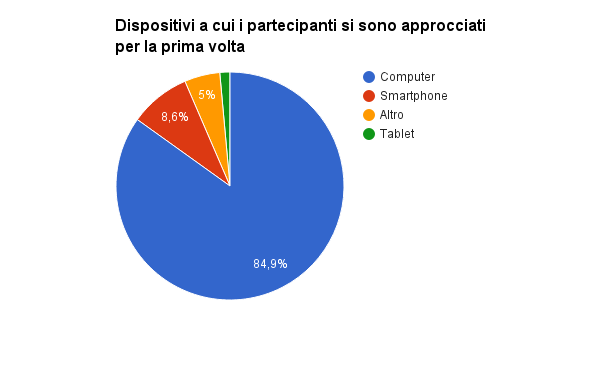
\includegraphics[scale=0.6]{img/chart_tipo_primo_approccio_dispositivi}
\end{figure}

\begin{quote}
	\textbf{Quanto ti ritieni competente con l'utilizzo di
	computer/smartphone?}
\end{quote}

Per valutare la competenza tecnologica sono state quindi poste all'utente,
tramite scala Likert a 5 valori (da per niente a moltissimo),
due domande di autovalutazione del suo livello di utilizzo di device
quali smartphone e computer.
\\
È abbastanza semplice notare, in entrambe le scale di valutazione,
come gli utenti si affermino su un livello
medio-alto, con una maggioranza sui valori $3$ e $4$.
\begin{figure}[H]
\centering
\begin{minipage}{.48\textwidth}
	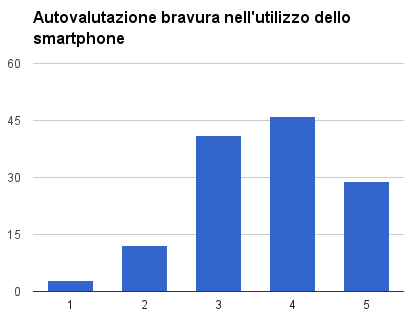
\includegraphics[scale=0.45]{img/chart_bravura_smartphone}
\end{minipage}
\hfill
\begin{minipage}{.49\textwidth}
	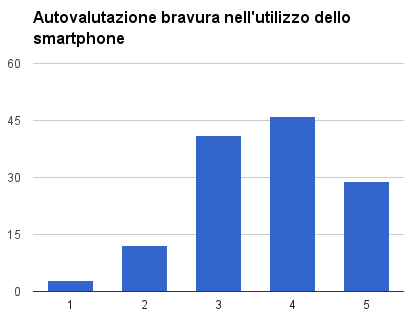
\includegraphics[scale=0.45]{img/chart_bravura_smartphone}
\end{minipage}
\end{figure}

\begin{quote}
	\textbf{Hai un problema al PC/telefono cellulare, che fai?}
\end{quote}

Al fine di inquadrare l'approccio degli utenti alla tecnologia, si è 
scelto di chiedere a questi ultimi come si comportino di fronte ai problemi con
i propri dispositivi. Le possibili risposte, in ordine decrescente di competenza da esse denotata
è:
\begin{itemize}
 \item Cerco di risolvere da solo;
 \item Cerco di capire e localizzare il problema per dare più informazioni possibili all'assistenza ma non tocco niente;
 \item Chiamo l'assistenza o un amico;
 \item Lo butto e ne compro un altro.
\end{itemize}

La maggior parte degli utenti intervistati dimostra intraprendenza: più dei due terzi cercano almeno di comprendere
il problema da soli, mentre più della metà tenta addirittura di risolvere i problemi.

\begin{figure}[H]
	\centering
	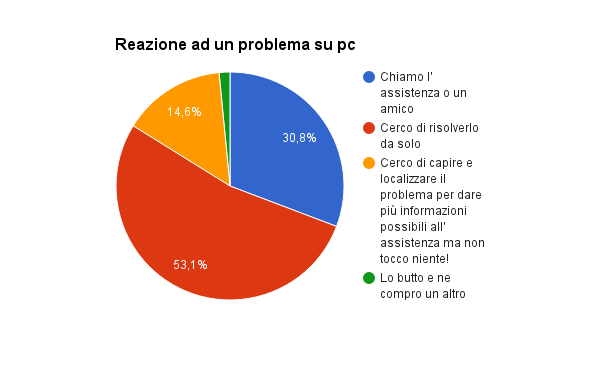
\includegraphics[scale=0.6]{img/chart_reazione_problema_pc}
\end{figure}

\subsubsection{Domande relative alla capacità culinaria}

\begin{quote}
	\textbf{Quanto ti ritieni competente in cucina?}
\end{quote}

Utilizzando una scala Likert con valori fra 1 e 5 è stato chiesto agli utenti di valutare la propria competenza culinaria.
Tale informazione è utile a inquadrare gli utenti rispetto alla loro competenza specifica di dominio. Un cuoco esperto, infatti,
avrà di certo requisiti diversi da uno alle prime armi.
\\
La distribuzione delle autovalutazioni ricalca una distribuzione normale con media 3. Gli utenti si divido infatti in modo
pressoché uniforme fra utenti competenti e utenti che non sono abili in cucina.


\begin{figure}[H]
	\centering
	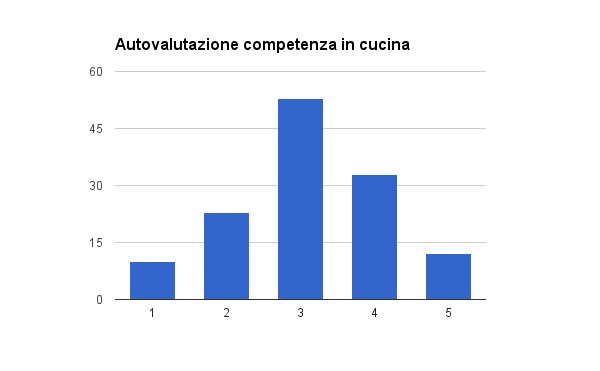
\includegraphics[scale=0.6]{img/chart_bravura_cucina}
\end{figure}

\begin{quote}
	\textbf{Degli amici si auto-invitano a casa tua per una cena, che fai?}
\end{quote}

Come nel caso della domanda precedente, anche in questo caso viene parzialmente misurata l'affinità degli utenti con la cucina.
Oltre a tale aspetto, si vuole comprendere quale sia l'approccio degli utenti all'improvvisazione culinaria, oltretutto
nel caso in cui si debba cucinare non solo per sé stessi. Le risposte possibili da noi previste sono le seguenti:
\begin{itemize}
 \item Inizio a sperimentare ai fornelli, voglio sorprendere tutti;
 \item Cerco qualche ricetta facile per stasera;
 \item Vado al supermercato per cercare qualcosa di semi pronto;
 \item Ordino qualcosa.
\end{itemize}

Dai risultati ottenuti la maggior parte (circa il 75\%) degli utenti è pronta a improvvisare una cena anche per i propri amici, mostrando
iniziativa e la volontà di cucinare per altri. Fra questi ultimi, la maggioranza cerca ricette facili, caso d'uso molto affine
ad un'applicazione di supporto alla cucina.

\begin{figure}[H]
	\centering
	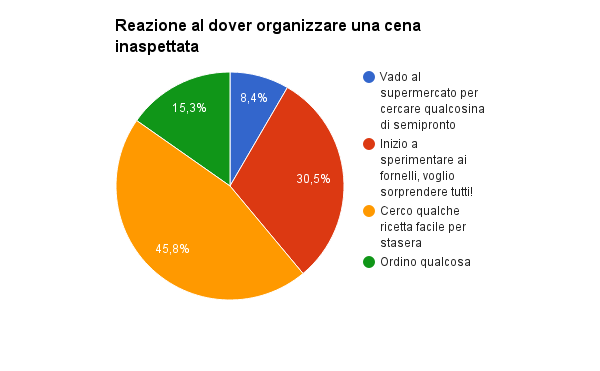
\includegraphics[scale=0.6]{img/chart_reazione_cena}
\end{figure}

\begin{quote}
	\textbf{Dove fai la spesa?}
\end{quote}
Il luogo o i luoghi nei quale viene effettuata la spesa da parte degli utenti. Tale informazione è doppiamente utile: da una parte,
è certamente correlata al ceto sociale di appartenenza, dall'altra, ci da informazioni sul livello di passione per il cibo del soggetto.
Le opzioni da noi previste sono:
\begin{itemize}
 \item Direttamente dal produttore al mercato;
 \item Ordino la spesa online;
 \item Piccoli commercianti;
 \item Supermercato.
\end{itemize}
Come era del resto prevedibile, la stragrande maggioranza degli utenti utilizzano i supermercati come fonti di cibo, mentre sono in minoranza quelli che
scelgono le altre opzioni. Questa informazione ci aiuta a comprendere come si possano aiutare gli utenti nell'effettuare la spesa.

\begin{figure}[H]
	\centering
	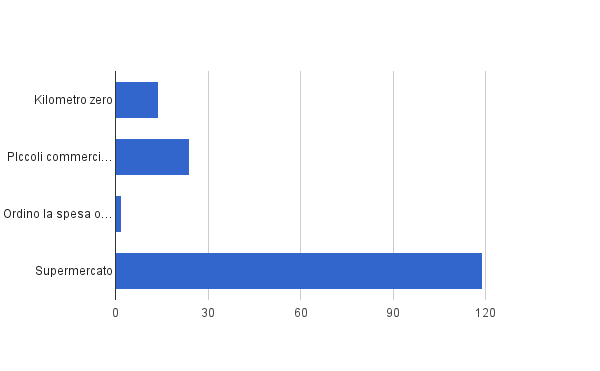
\includegraphics[scale=0.6]{img/chart_dove_fai_la_spesa}
\end{figure}

\begin{quote}
	\textbf{Hai allergie o intolleranze al cibo?}
\end{quote}

Con questa domanda si intende valutare l'impatto di allergie varie sulla popolazione totale. Si è scelto inoltre di contare chi ha intolleranze multiple.
Dai risultati ottenuti emerge come l'impatto di allergie sulla popolazione sia minoritario ma non trascurabile.

\begin{figure}[H]
	\centering
	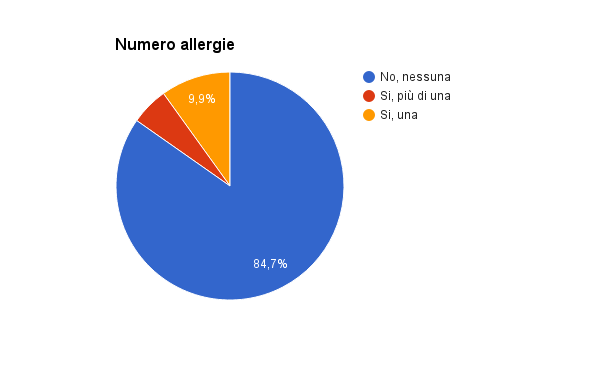
\includegraphics[scale=0.6]{img/chart_allergie}
\end{figure}

\begin{quote}
	\textbf{Usi app o siti web per cucinare? Se hai risposto no, ti interesserebbe un'app per cucinare?}
\end{quote}

Tramite tali domande si intende valutare da una parte la diffusione di software per l'ausilio alla cucina, dall'altra
l'interesse per un'eventuale applicazione fra chi non utilizza tali software. La maggior parte degli utenti utilizza un applicazione,
chi non utilizza strumenti software è in gran parte interessato ad una applicazione di questo tipo.

\begin{figure}[H]
\centering
\begin{minipage}{.48\textwidth}
	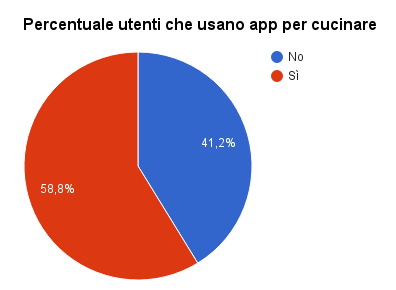
\includegraphics[scale=0.45]{img/chart_usi_app_cucina}
\end{minipage}
\hfill
\begin{minipage}{.49\textwidth}
	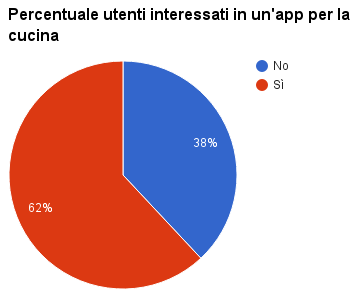
\includegraphics[scale=0.45]{img/chart_vorresti_app_cucina}
\end{minipage}
\end{figure}

\begin{quote}
	\textbf{Usi app o siti web per fare la spesa? Se hai risposto no, ti interesserebbe un'app per fare la spesa?}
\end{quote}

Come nel caso precedente, si vuole misurare l'utilizzo e l'interesse verso un'applicazione che aiuti gli utenti a fare
la spesa. Dai risultati emerge uno scarso utilizzo di applicazioni per fare la spesa, nonché un interesse molto meno marcato
che nel caso della domanda precedente.

\begin{figure}[H]
\centering
\begin{minipage}{.48\textwidth}
	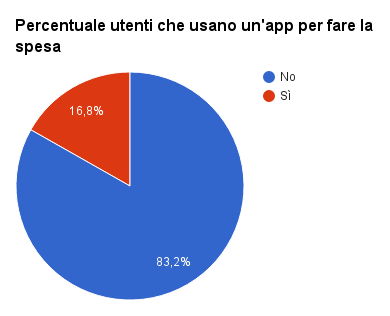
\includegraphics[scale=0.45]{img/chart_usi_app_spesa}
\end{minipage}
\hfill
\begin{minipage}{.49\textwidth}
	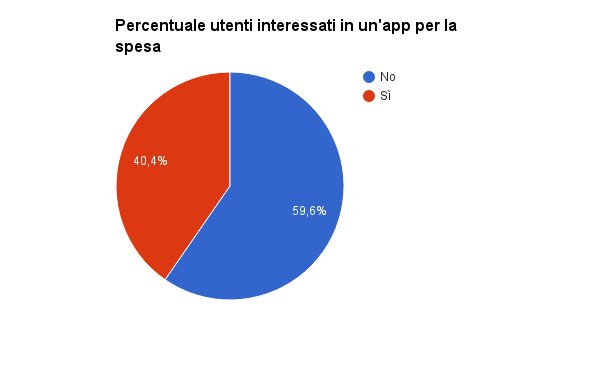
\includegraphics[scale=0.45]{img/chart_vorresti_app_spesa}
\end{minipage}
\end{figure}

\subsection{Analisi combinata dei dati}
Per ottenere una migliore profilazione degli utenti si è optato per combinare i
dati precedentemente presentati nel seguente modo:

\begin{quote}
	\textbf{Competenze digitali per fascia d'età}
\end{quote}
I dati sono stati combinati per ottenere maggiori informazioni a riguardo
dell'utilizzo da parte degli utenti degli smartphone, come è possibile intuire
facilmente, la maggior parte dei giovani è molto capace con lo smartphone,
mentre la maggior parte delle persone in età avanzata si attesta su valori
bassi, le persone nelle fasce intermedie si sono dichiarate degli utilizzatori
``normali" per quanto riguarda l'utilizzo di smartphone e computer.
\begin{figure}[H]
\centering
	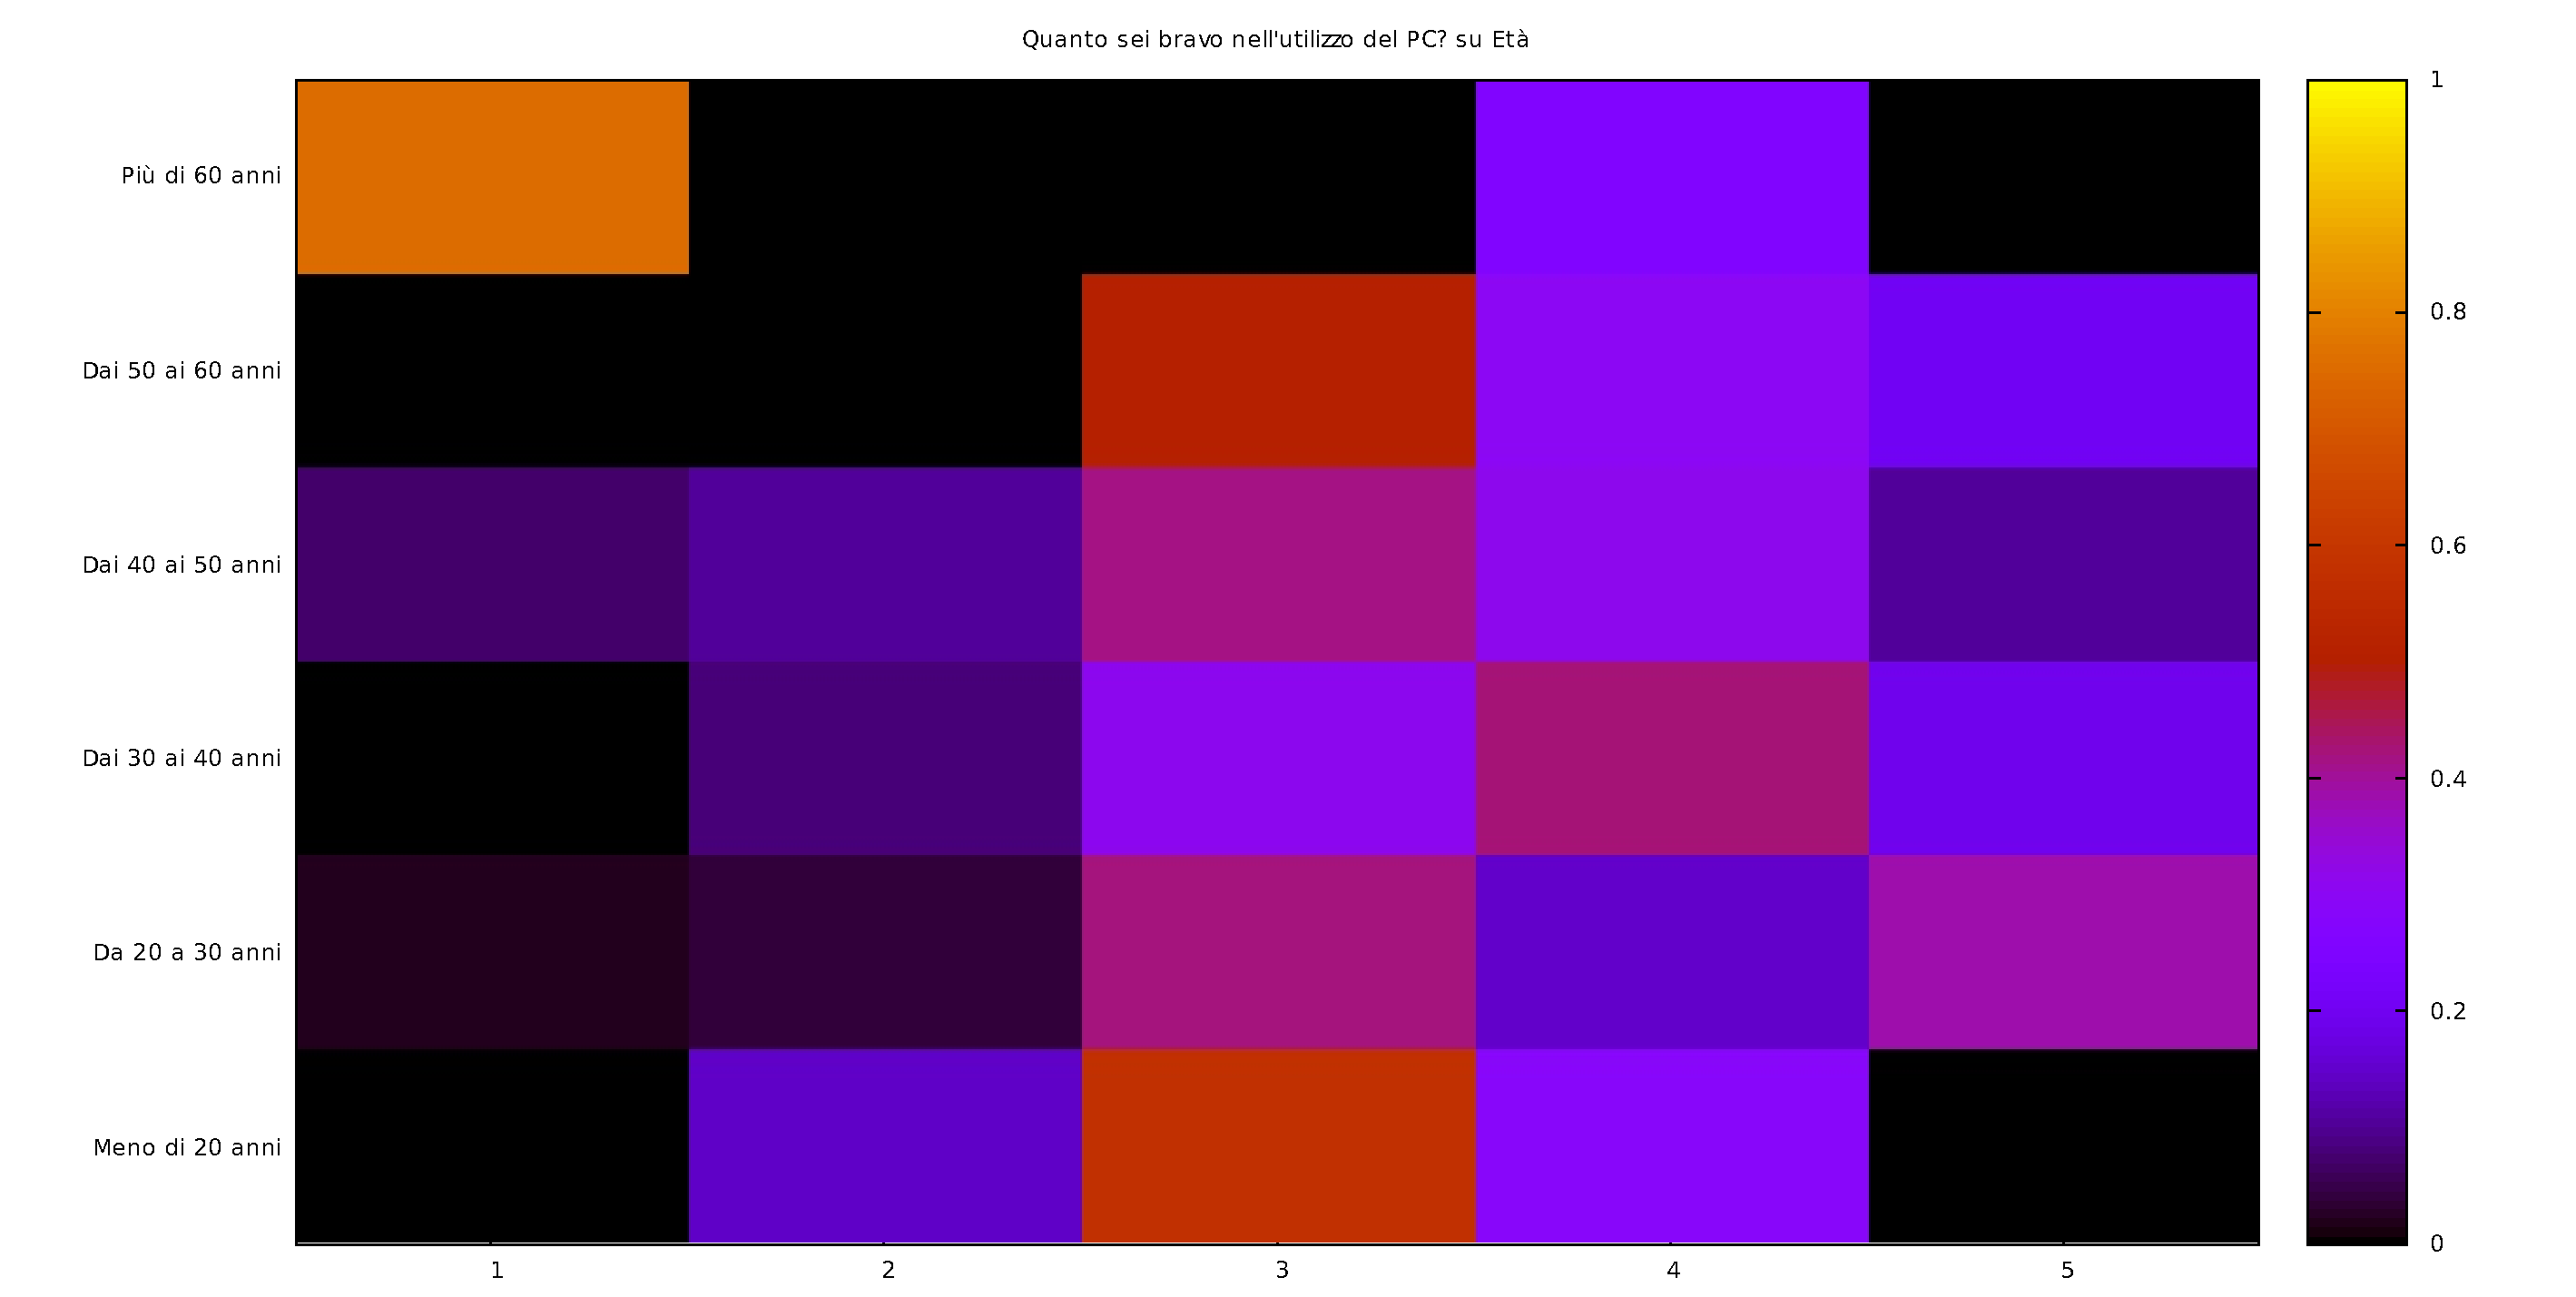
\includegraphics[width=\textwidth]{img/heatmap_pc_eta}
\end{figure}
\begin{figure}[H]
	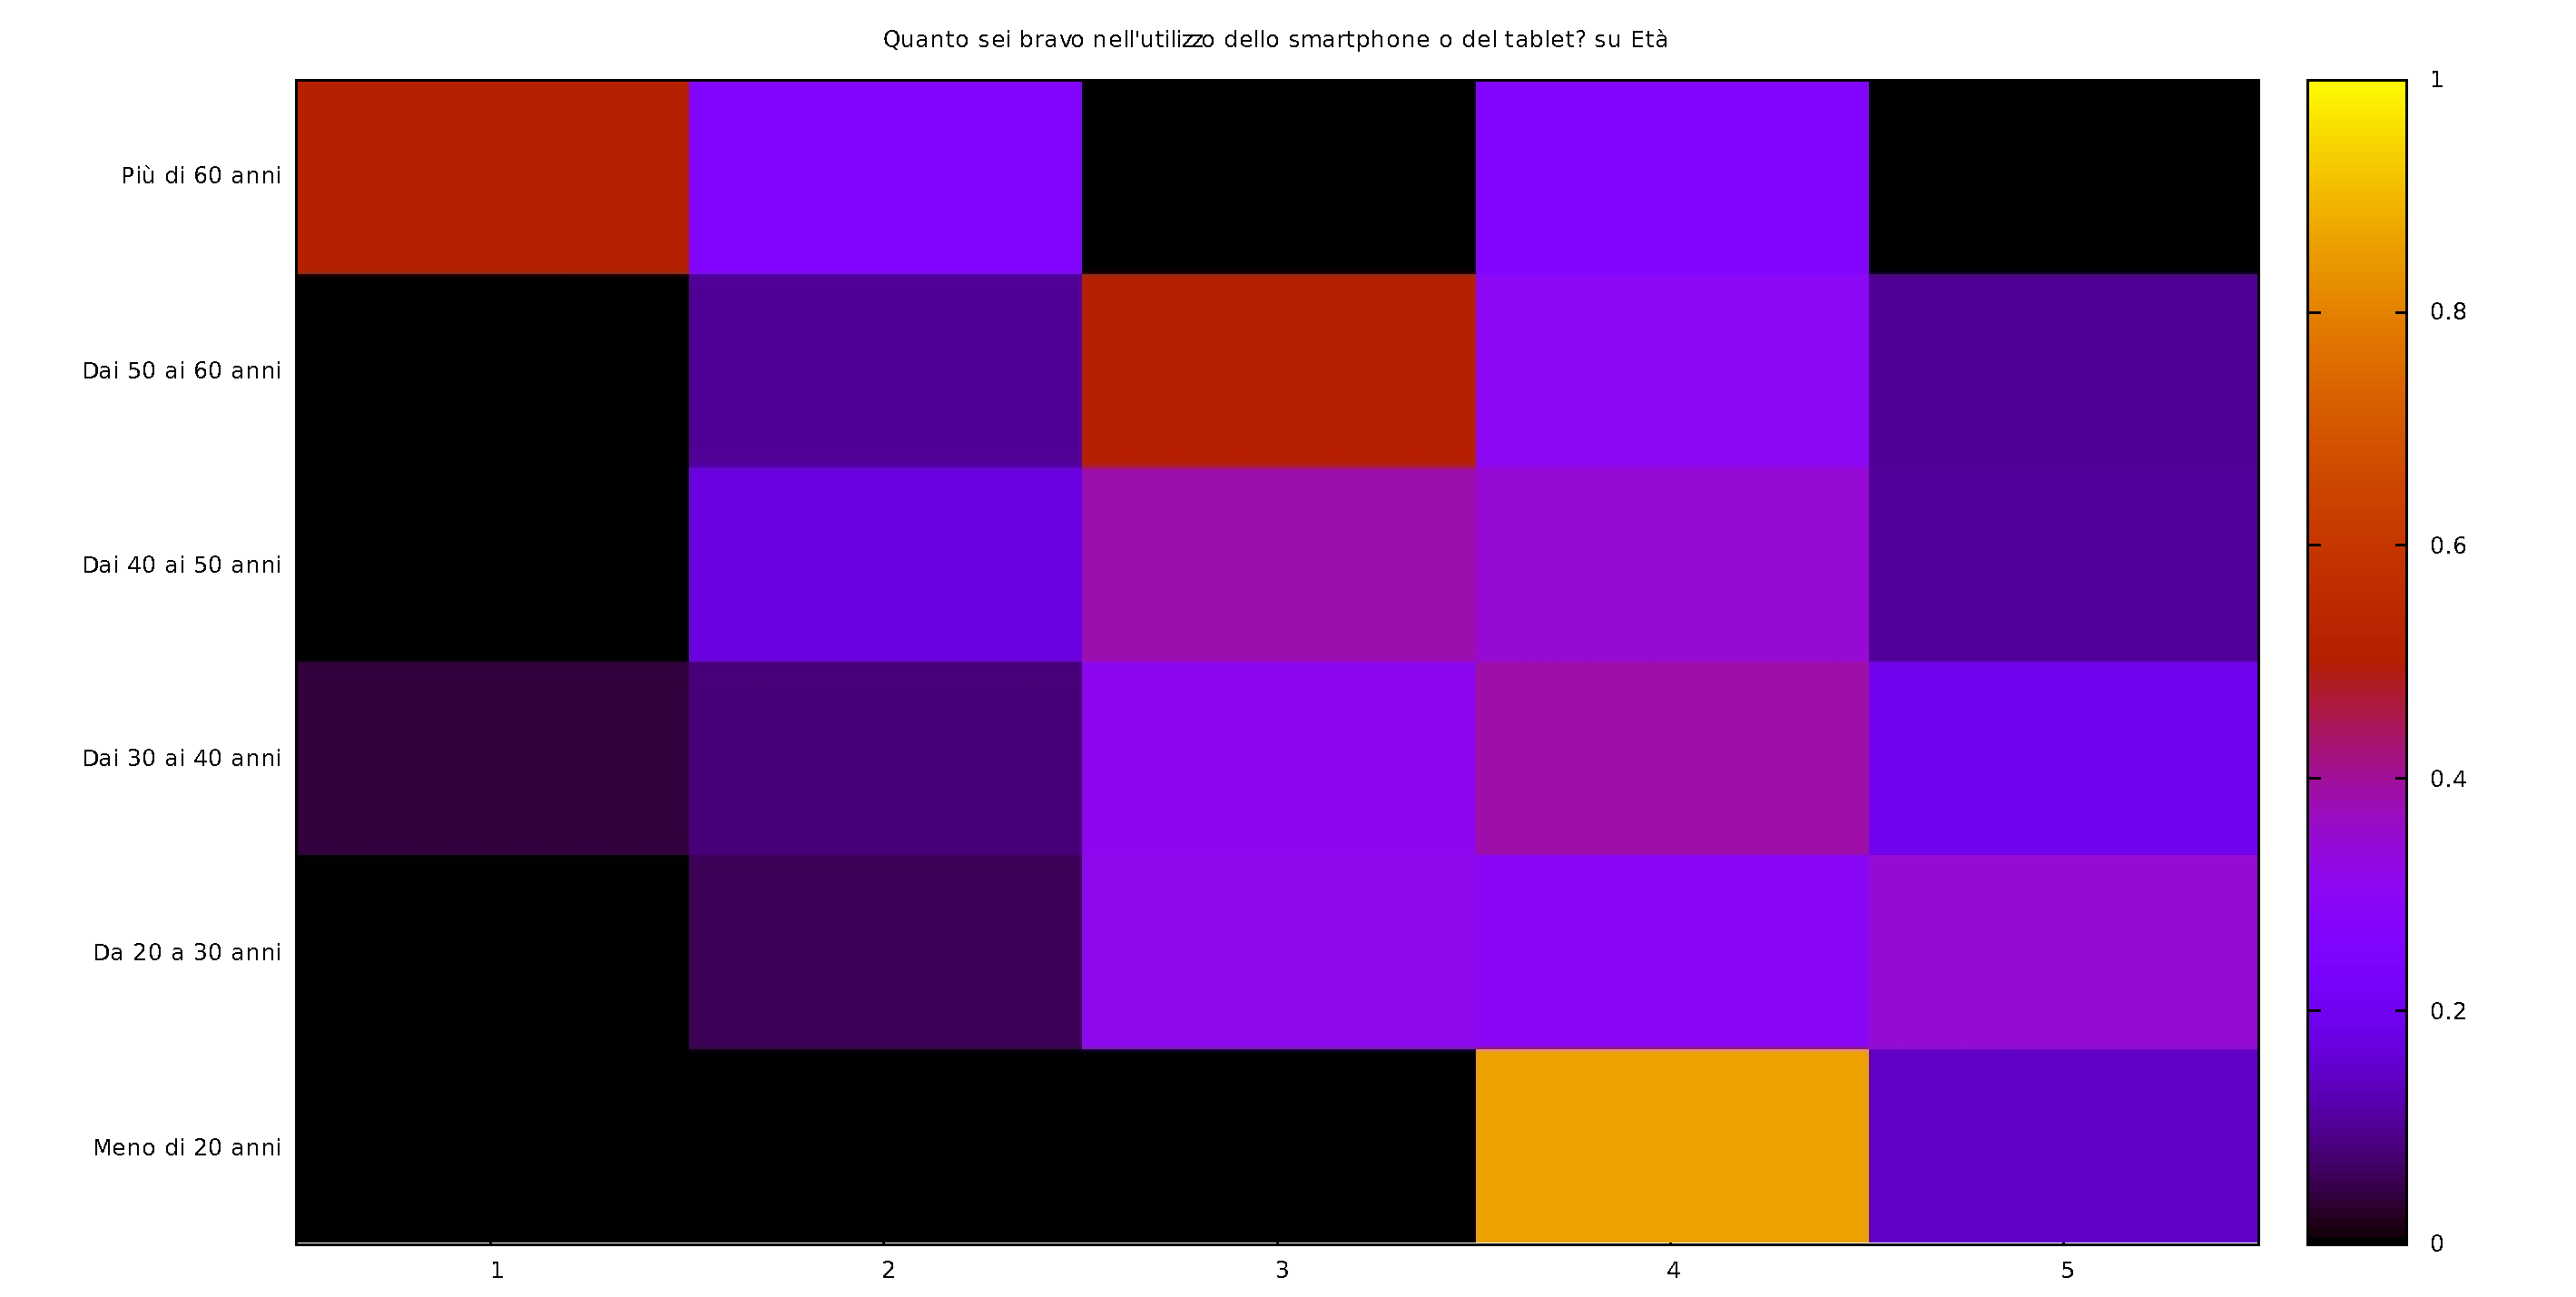
\includegraphics[width=\textwidth]{img/heatmap_smartphone_eta}
\end{figure}


\begin{quote}
	\textbf{Autovalutazione della bravura in cucina con o senza l'utilizzo
	di applicazioni}
\end{quote}
È stata inoltre valutata la capacità reale degli utenti con il quale ci si
rapporterà, ottenendo dati a riguardo di un'effettiva miglioria apportata da
un'eventuale applicazione negli utenti e gli interesse degli stessi nel
utilizzarla.\\
L'analisi dei dati ha prodotto risultati notevolmente a favore per l'utilizzo di
un'applicazione, attestandosi su valori più alti per persone facenti uso di
questo genere di programmi.
\begin{figure}[H]
	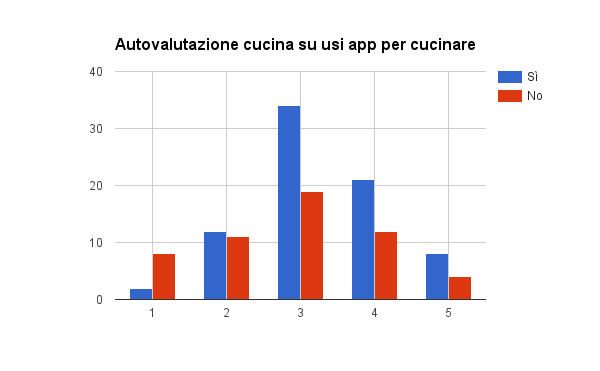
\includegraphics[width=\textwidth]{img/chart_autovalutazione_e_usi_app}
\end{figure}
